%本章では,提案手法である ID の連続性を意識した Sequential と
%演算時のアクセス局所性を意識した DBG Early Estimation (DBG-EE) についてそれぞれ説明する.
本研究では,グラフを取得しながらノード ID を再配置する手法として,Sequential と DBG Early Estimation (DBG-EE) を提案する.
図\ref{research_position} で示すように,Sequential は ID の連続性を意識し,DBG-EE は演算時のアクセス局所性を意識している.
Sequential では ID の連続性を保証するために RW で出会ったノード順に昇順の連続した ID を再配置する.
DBG-EE では 図\ref{degree_appro} で示すように,RW 途中での取得グラフにおける次数分布が RW 終了時点の取得グラフにおける次数分布に近似する性質に着目し ID を再配置する.
具体的には,既存手法でノードの次数情報しか必要とせず,前処理コストと演算速度向上のバランスに優れる DBG \cite{faldu2019closer} をもとに再配置を行う.
\begin{figure}[t]
  \centering
  %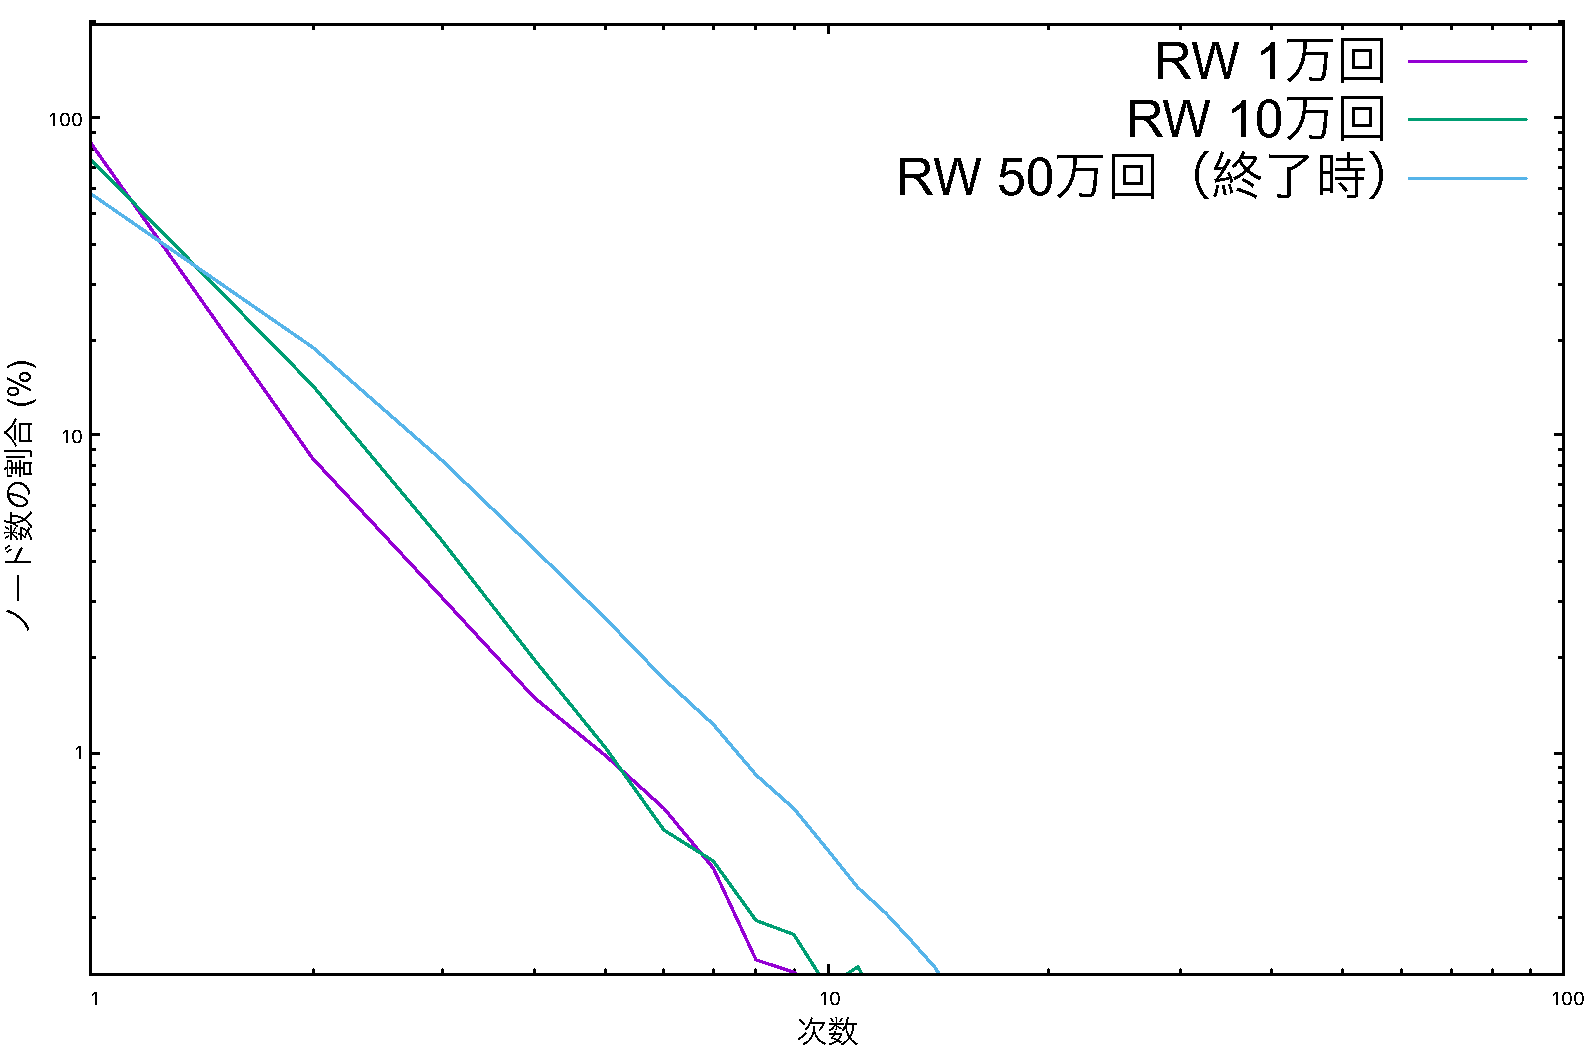
\includegraphics[width=\linewidth]{./figure/degree_dist.pdf}
  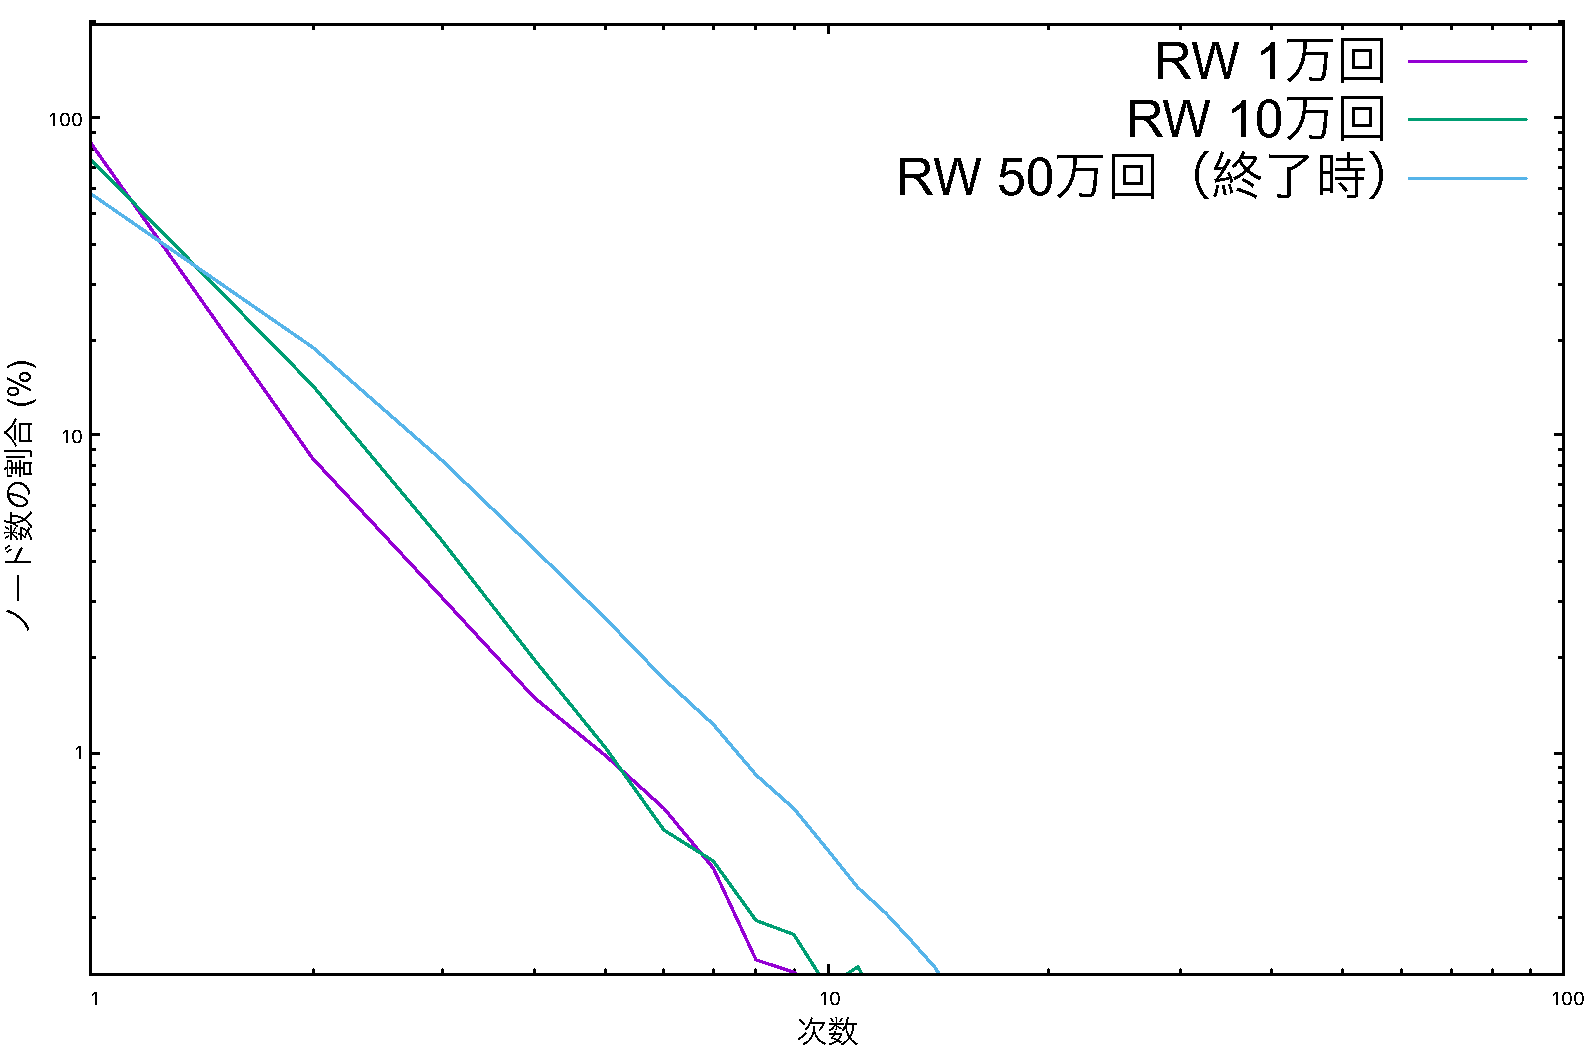
\includegraphics[width=12cm]{./figure/degree_dist.pdf}
  \caption{取得途中のグラフと取得完了時のグラフにおける次数分布}
  \label{degree_appro}
\end{figure}
\section{Sequential}
Sequential では,RW によるグラフ取得において新しく出会ったノード順に連続した昇順の ID を再配置する.
再配置に伴い新たな ID が割り振られる度に,元の ID と新たな ID の対応関係をマッピングテーブルへ登録する.
このマッピングテーブルを参照することで,RW 途中での訪問先ノードがすでに再配置済みか即座に判定することが可能となっている.

\subsection{RW の訪問順に基づく ID 再配置}
Sequential による ID 再配置の具体例を 図\ref{sequential-rw} で示すように 1 → 4 の順でノードを移動しグラフを取得する場合で考える.
このとき,図\ref{sequential} に示す手順で ID の再配置と再配置済みグラフの更新が行われる.
まず,RW 開始時点で再配置されたノードは存在しないため,1回目の移動に伴い ID 10 の始点ノードと ID 6 のノードに
それぞれ ID 0 と ID 1 が再配置される.
そして,ID 10 → ID 0,ID 6 → ID 1 という対応関係をマッピングテーブルに登録し,ID 0 のノードと ID 1 のノード間にエッジが張られていることを再配置済みのグラフ構造として保持する.
次に,2回目の移動に伴い ID 37 というノードへ辿り着くが,マッピングテーブルに ID 37 の対応関係は登録されていない.
そこで,新たに ID 37 のノードへ ID 2 を再配置し,ID 37 → ID 2 という対応関係をマッピングテーブルへ登録する.
そして,マッピングテーブルの参照により ID 6 → ID 1,ID 37 → ID 2 という対応関係が分かるので,ID 1 のノードと ID 2 のノード間にエッジが張られていることを再配置済みのグラフへ反映させる.
以降も同様にマッピングテーブルの参照・登録及び再配置済みグラフの更新を RW 終了まで繰り返す.
\begin{figure}[t]
  \centering
  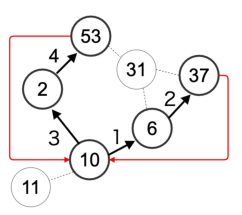
\includegraphics[width=7cm]{./figure/sequential-rw.pdf}
  \caption{1→4 の順にノードを移動しグラフを取得}
  \label{sequential-rw}
\end{figure}
\begin{figure}[t]
  \centering
  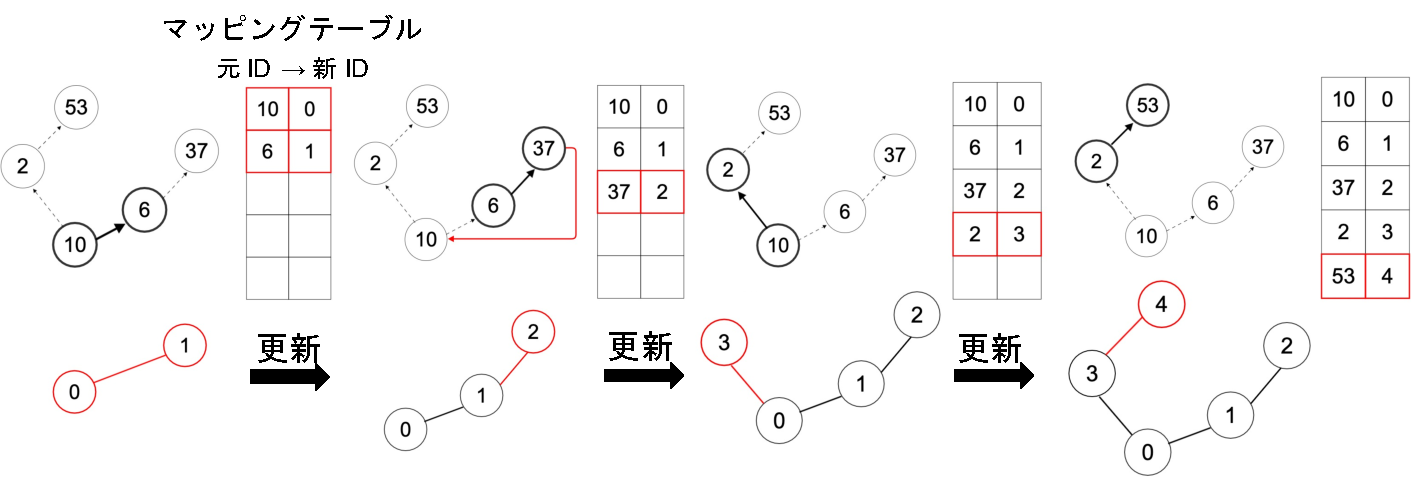
\includegraphics[width=\linewidth]{./figure/sequential.pdf}
  \caption{Sequential におけるノード ID 再配置}
  \label{sequential}
\end{figure}

\subsection{メモリ使用量を抑えたグラフ構造の保持}
Sequential では RW でノードを移動する度にマッピングテーブルの参照・登録及び再配置済みグラフの更新を行うことで
再配置待ちのグラフ構造を保持する必要を無くし,メモリ使用量を削減している.
図\ref{sequential_bad_memory}で示すように,グラフを取得してから再配置を行う場合は取得完了時のグラフと再配置済みのグラフを
メモリ上で保持する必要がある.
しかし,Sequential による再配置では図\ref{sequential_good_memory}で示すように,RW で移動した1エッジと再配置済みのグラフを保持するだけで良く,
1エッジを保持するためのメモリ使用量は取得完了時のグラフを保持するためのメモリ使用量より遥かに小さい.
\begin{figure}[t]
  \begin{tabular}{cc}
    \begin{minipage}[t]{0.45\hsize}
      \centering
      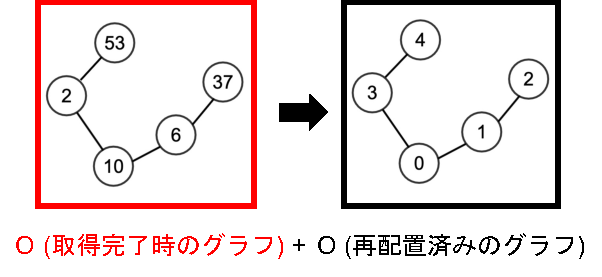
\includegraphics[width=7cm]{./figure/sequential_bad_memory.pdf}
      \caption{取得が完了してから再配置する場合の\\メモリ使用量}
      \label{sequential_bad_memory}
    \end{minipage} &
    \begin{minipage}[t]{0.45\hsize}
      \centering
      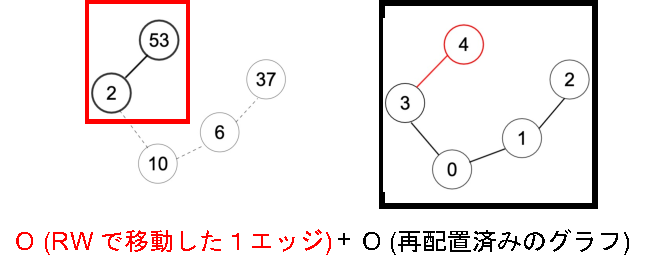
\includegraphics[width=7cm]{./figure/sequential_good_memory.pdf}
      \caption{Sequential において再配置に必要な\\メモリ使用量}
      \label{sequential_good_memory}
    \end{minipage}
  \end{tabular}
\end{figure}
\subsection{近接構造による局所性の部分的な実現}
Sequential は RW によるグラフ取得の途中で出会ったノード順に連続した ID を再配置するため ID の連続性は保証される.
さらに,RW では始点に戻る場合を除き,隣接ノードにしか移動しないため,図\ref{sequential-rw}で示す 1 → 2 のような移動の場合,
隣接ノードへ連続した ID が再配置される.
このように,Sequential では RW による移動の仕方によって隣接ノードへ連続した ID の再配置が可能となり,
近接構造によるアクセス局所性を考慮した再配置が部分的に実現されている.

\section{DBG Early Estimation (DBG-EE)}
DBG-EE は RW によるグラフ取得の途中でノードを次数に基づきグループ分けし,各グループ毎に ID を再配置する.
なお,DBG-EE では DBG におけるグループ定義を踏襲し,グラフの平均次数$\mathbb{A}$に基づき,[0,$\mathbb{A}$/2),[$\mathbb{A}$/2,$\mathbb{A}$),[$\mathbb{A}$,2$\mathbb{A}$),[2$\mathbb{A}$,4$\mathbb{A}$),
[4$\mathbb{A}$,8$\mathbb{A}$),[8$\mathbb{A}$,16$\mathbb{A}$),[16$\mathbb{A}$,32$\mathbb{A}$),[32$\mathbb{A}$,$\infty$)
と 8 グループを定義する.
以下,簡単のため [32$\mathbb{A}$,$\infty$) をグループ 0,[16$\mathbb{A}$,32$\mathbb{A}$) をグループ 1,[8$\mathbb{A}$,16$\mathbb{A}$) をグループ 2,[4$\mathbb{A}$,8$\mathbb{A}$) をグループ 3,
[2$\mathbb{A}$,4$\mathbb{A}$) をグループ 4,[$\mathbb{A}$,2$\mathbb{A}$) をグループ 5,[$\mathbb{A}$/2,$\mathbb{A}$) をグループ 6,[0,$\mathbb{A}$/2) をグループ 7 と呼ぶ.
DBG では図\ref{dbg} で示すように,ノードのグループ分けが完了してから ID の再配置を実行する.
しかし,グラフ取得が完了するまで各グループに属するノード数は未定であるため,DBG と同様にグループ 0 から順に ID を再配置することは不可能である.
取得完了時の各グループサイズが未定な状況でグラフを取得しながら ID を再配置するには,予め各グループが再配置に使用する ID の範囲を定めておく必要がある.
そこで,DBG-EE では取得初期の段階で各グループのグループサイズを推定し,推定したサイズに基づいて各グループが再配置に使用する ID の範囲を決定する.
また,グラフの取得途中で再配置を実行し,再配置済みのグラフへ反映が完了した時点で取得したグラフを破棄することで,
取得完了まで再配置待ちのグラフを保持し続ける必要が無くなり,メモリ使用量が削減される.
さらに,グラフ取得と ID の再配置を並列して行うことで,グラフ取得を待つだけの時間を減少させ,時間コストを削減させている.

\subsection{グループサイズの早期推定}
DBG-EE では,グラフ取得のために RW を N 回実行する中で RW M 回毎に ID の再配置を実行する.
つまり,再配置は全体で N/M 回実行されるため,1 回目の再配置を実行する段階で各グループが N/M 回の再配置実行時に使用する ID の範囲を決定する必要がある.
そこで,DBG-EE では1回目の再配置実行時のグループ分け結果に基づき各グループサイズを N/M 倍し,その値を各グループの推定サイズとみなす.
なお,グループ分けを実行する際には取得途中のグラフにおける平均次数を使用する.
図\ref{degree_appro} で示すように,RW 回数が少ない段階での取得グラフにおける次数分布は RW 回数が増加した場合の次数分布に良く近似する.
そのため,取得途中のグラフにおける平均次数に基づきノードをグループ分けすることは有効であり,\ref{sec:dbg} で述べた次数による局所性と近接構造による局所性が考慮される ID の再配置が可能である.
図\ref{estimation_size} にグラフサイズ推定の例を示す.
1 回目のグループ分けにより X 個のノードがグループ0へ割り振られた場合,グループ0の推定サイズは X * N/M となる.
同様に他グループでも 1 回目のグループ分けにより割り振られたノード数を N/M 倍し,グループサイズを推定する.

\begin{figure}[t]
  \centering
  %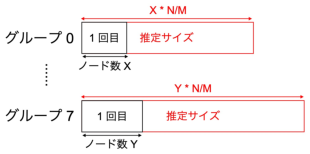
\includegraphics[width=\linewidth]{./figure/estimated_group_size.pdf}
  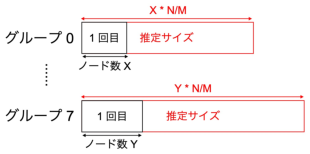
\includegraphics[width=12cm]{./figure/estimated_group_size.pdf}
  \caption{グループサイズの早期推定}
  \label{estimation_size}
\end{figure}
\subsection{推定サイズに基づく ID の範囲決定}
1 回目のグループ分け結果に基づき各グループサイズを推定した後,推定サイズに基づいた ID の範囲決定を行う.
推定サイズに基づく ID の範囲決定の様子を図\ref{group_id_range} に示す.
まず,最も高次数のノードが属するグループ 0 に ID 0 からグループ 0 の推定サイズまでの範囲を与える. 
次に,グループ 1 にはグループ 0 の範囲が終了した点からグループ 1 の推定サイズまでの範囲を与える.
同様に他グループにも前グループの範囲が終了した点から推定サイズまでの範囲を与える.
\begin{figure}[t]
  \centering
  %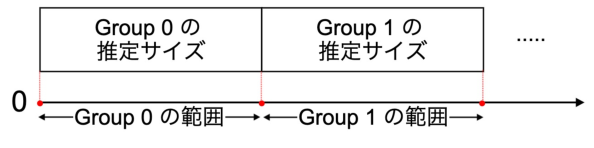
\includegraphics[width=\linewidth]{./figure/group_id_range.pdf}
  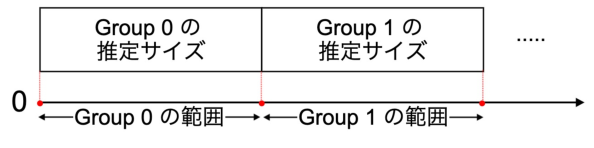
\includegraphics[width=12cm]{./figure/group_id_range.pdf}
  \caption{推定サイズに基づく ID の範囲決定}
  \label{group_id_range}
\end{figure}
ID の範囲決定後は RW M 回毎に取得したグラフでグループ分けを実行し,各グループの範囲において ID の再配置が済んでいないノードに新たな ID を再配置する.
なお,再配置を実行する際,各グループは範囲内で最小の ID から順に使用する.
例えば,1 回目の再配置でグループ 0 に 10 個のノードが割り振られた場合,これらのノードには 0 ~ 9 の ID が再配置される. 
次に 2 回目の再配置を実行する時,グループ 0 の範囲内で最小の ID は 10 なので,グループ 0 に割り振られたノードには 10 以降の ID が再配置される.
この時,RW によるグラフ取得が完了し,全てのノードに対して ID 再配置が完了した段階で,図\ref{dbg-ee_not_consecutive} で示すように,範囲内全ての ID が使用されないとグループ間で ID の連続性が失われてしまう.
\begin{figure}[t]
  \centering
  %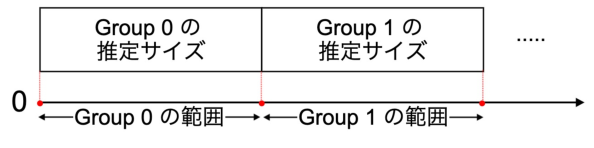
\includegraphics[width=\linewidth]{./figure/group_id_range.pdf}
  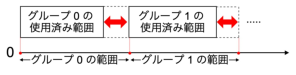
\includegraphics[width=12cm]{./figure/dbg-ee_not_consecutive.pdf}
  \caption{グループ間で ID の連続性が欠如する場合}
  \label{dbg-ee_not_consecutive}
\end{figure}

\subsection{部分的な取得グラフの破棄}
図\ref{dbg-ee_bad_memory} で示すようにグラフを取得してから ID を再配置する場合,\ref{sequential_bad_memory} で示した Sequential の場合と同様に
取得完了時のグラフサイズに応じた余分な空間コストが発生する.
そこで DBG-EE では,図\ref{dbg-ee_good_memory} で示すように,再配置済みグラフへの反映が完了した段階で取得したグラフを破棄する.
これにより,RW によるグラフ取得が完了するまで ID 再配置待ちのグラフ構造を保持し続ける必要が無くなり,空間コストが減少する.
しかし,Sequential では RW で移動した 1 エッジのみ保持すれば十分であるという点と比べると,Sequential より空間コストの減少は小さい.
また,再配置を実行する間隔 M の値が大きいほど,取得途中でより巨大なグラフを保持する必要があるため空間コストは増加する.
\begin{figure}[t]
  \centering
  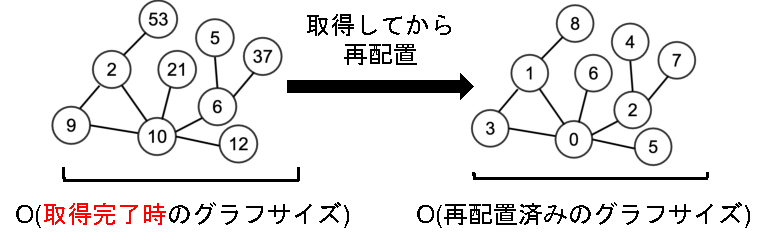
\includegraphics[width=\linewidth]{./figure/dbg-ee_bad_memory.pdf}
  \caption{取得完了してから再配置する場合のメモリ使用量}
  \label{dbg-ee_bad_memory}
\end{figure}
\begin{figure}[t]
  \centering
  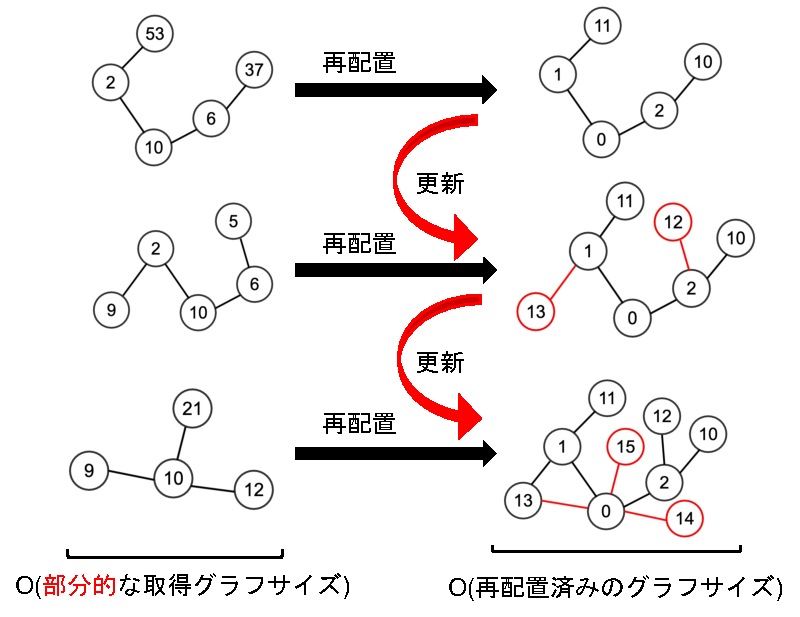
\includegraphics[width=\linewidth]{./figure/dbg-ee_good_memory.pdf}
  \caption{DBG-EE におけるメモリ使用量}
  \label{dbg-ee_good_memory}
\end{figure}

\subsection{グラフ取得と再配置の並列処理}
グラフの取得が完了してから ID を再配置する場合では,グラフ取得を待つだけの無駄な時間が発生してしまう.
そこで DBG-EE では,図\ref{dbg-ee_para} で示すように,グラフ取得の完了を待ってから ID 再配置を行うのではなく,
グラフ取得の待ち時間中に ID の再配置を完了させておくことで時間コストを削減している.
\begin{figure}[t]
  \centering
  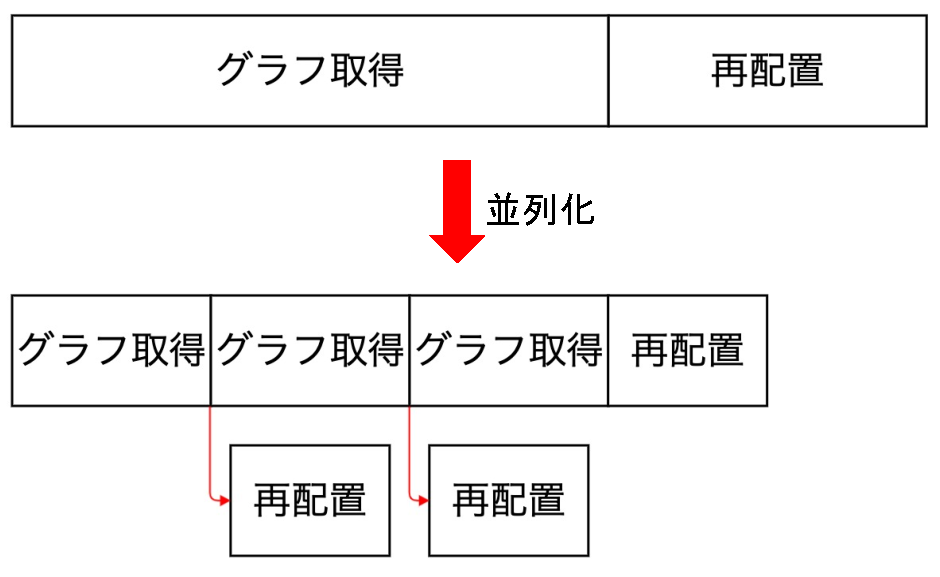
\includegraphics[width=0.8\linewidth]{./figure/dbg-ee_para.pdf}
  \caption{グラフ取得と再配置の並列処理}
  \label{dbg-ee_para}
\end{figure}